\documentclass[12pt,a4paper,openright,twoside]{book}
\usepackage[utf8]{inputenc}
\usepackage{disi-thesis}
\usepackage{code-lstlistings}
\usepackage{notes}
\usepackage{shortcuts}
\usepackage{acronym}
\usepackage[acronym]{glossaries}

\school{\unibo}
\programme{Corso di Laurea Triennale in Ingegneria e Scienze Informatiche}
\title{DGA Domain Generation Algorithm}
\author{Simone Collorà}
\date{\today}
\subject{Programmazione a Oggetti}
\supervisor{Prof. Mirko Viroli}
\cosupervisor{Dott. CoSupervisor 1}
\morecosupervisor{Dott. CoSupervisor 2}
\session{I}
\academicyear{2024-2025}

% Definition of acronyms
\acrodef{IoT}{Internet of Thing}
\acrodef{vm}[VM]{Virtual Machine}
\newacronym{DGA}{DGA}{Domain Generation Algorithm}
\newacronym{C&C}{C\&C}{Command and Control}


\mainlinespacing{1.241} % line spacing in mainmatter, comment to default (1)

\begin{document}

\frontmatter\frontispiece

\begin{abstract}	
Max 2000 characters, strict.
\end{abstract}

\begin{dedication} % this is optional
Optional. Max a few lines.
\end{dedication}

%----------------------------------------------------------------------------------------
\tableofcontents   
\listoffigures     % (optional) comment if empty
\lstlistoflistings % (optional) comment if empty
%----------------------------------------------------------------------------------------

\mainmatter

%----------------------------------------------------------------------------------------
\chapter{Introduction}
\label{chap:introduction}
%----------------------------------------------------------------------------------------

Write your intro here.
%\sidenote{Add sidenotes in this way. They are named after the author of the thesis}

La sicurezza informatica è un argomento di crescente importanza
nel mondo moderno. Con il passare del tempo,
i sistemi di protezione sono diventati sempre più sofisticati
e potenti ma allo stesso tempo anche gli hackers 
hanno sviluppato tecniche sempre più avanzate per eludere i sistemi di protezione.
Tra queste vi è sicuramente l'uso 
dei \acrfull{C&C} servers. I \acrshort{C&C} sono dei server che manipolano
i computer infetti da malwares, chiamati Botnets o Zombi, permettendo
all'attaccante di eseguire codice malevolo da remoto.
Il malware, però, deve conoscere un indirizzo IP o un dominio
per contattare il server. L'attaccante potrebbe
inserire in modo bruto l l'indirizzo IP del server nel codice del malware,
ma questo metodo è facilmente rilevabile e bloccabile.
Gli hackers, quindi, preferiscono utilizzare dei domini
generati in modo pseudo casuale per nascondere i loro server chiamati
\acrfull{DGA} servers.



\paragraph{Structure of the Thesis}

%\note{At the end, describe the structure of the paper}

\chapter{Background(nome provvisorio)}

I suggest referencing stuff as follows: \cref{fig:DGA example} or \Cref{fig:DGA example}

I \acrshort{DGA} sono algoritmi che generano domini in modo pseudo casuale.
Prima viene scelto un seed, di solito la data odierna
o le previsioni meteo \cite{8621875}
In questo modo, diventa più difficile per i sistemi di protezione
rilevare e bloccare i loro attacchi.
Si potrebbe pensare di bloccare direttamente i domini tramite
una blacklist ma questo metodo
risulta inefficace poiché vengono generati migliaia di domini
continuamente. Si pensi che Conficker C, un famoso malware
che utilizza \acrshort{DGA}, è in grado di generare
fino a 50.000 domini pseudo casuali al giorno \cite{978131}.
Un altro modo per contrastare ciò
potrebbe essere quello di fare reverse engineering
del \acrshort{DGA} per capire quale seed viene utilizzato per generare i domini.
Questo però risulta lento e dispendioso e possibilmente inefficace. \cite{8887881}


\begin{figure}
    \centering
    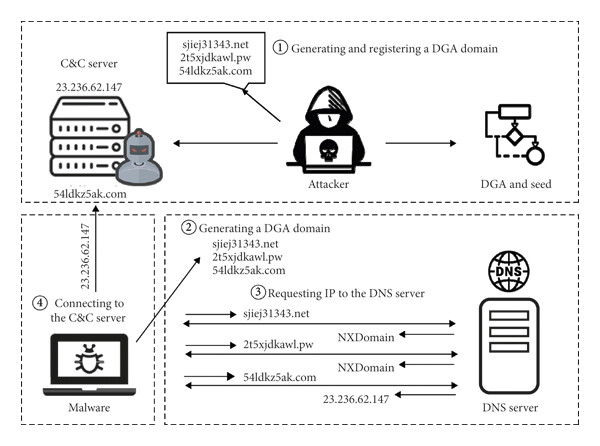
\includegraphics[width=.8\linewidth]{figures/DGA example.jpg}
    \caption{esempio del funzionamento di un \acrshort{DGA}}
    \label{fig:DGA example}
\end{figure}

\section{Some cool topic}

\chapter{Contribution}

You may also put some code snippet (which is NOT float by default), eg: \cref{lst:random-code}.

\lstinputlisting[float,language=Java,label={lst:random-code}]{listings/HelloWorld.java}

\section{Fancy formulas here}

%----------------------------------------------------------------------------------------
% BIBLIOGRAPHY
%----------------------------------------------------------------------------------------

\backmatter

\bibliographystyle{plain} %prima era alpha
\bibliography{bibliography}

\begin{acknowledgements} % this is optional
Optional. Max 1 page.
\end{acknowledgements}

\end{document}
